% Discuss the PEAR work and how it is relevant

\chapter{Physically Enhanced Authentication Ring}
\label{chapter:pear}

\section{Overview}
One problem that is present when using computers is that users typically are not aware of the security of the system
they are using. For instance, an attacker could have installed a key logger on a user's system to harvest every username
and password they have. Even with the best security systems on the machine in place, if the attacker is able to capture
a user's keystrokes, the other security is moot. 

PEAR, or Physically Enhanced Authentication Ring, was designed to counteract this key logger threat to a system. In addition
to defending against keyloggers specifically, it increases security in general because it is the second part of a "two factor
authentication" system. It also is a physical system, specifically a peripheral physical system, since it incorporates its
own processing and interacts with the user's normal computer system. Thirdly, the PEAR system incorporates a PUF device,
so it is a good example of when PUF technology is useful.

From a high level perspective, a PEAR device is a device consisting of a PUF, a keypad, and some supporting circuitry. When
a user wishes to log on to a given service, rather than using the keyboard for a password, he enters a 4 digit PIN on the PEAR
device. The PEAR device then executes the PUF and then initiates a zero-knowledge proof of knowledge with the service
provider. Note that no sensitive data is actually input to the PC, which potentially has a keylogger. Any data that the PC
is requested to ferry between the PEAR device and the service provider is encrypted, so recording this data does not reveal
any information.

The system works by having every service provider associated with an ID number of some kind. Each user of the service will
also have an ID number associated with it. This allows both parties to identify themselves to each other.

\section{Protocol Details}
The PEAR system consists of two parts, an enrollment step initially and then an authentication step.
Table~\ref{tab:pearprotocol} presents a formalized description of the protocols, while Figure~\ref{fig:pearauthentication}
and Figure~\ref{fig:pearenrollment} give graphical representations that occur.

An interesting point to note is that during the enrollment stage, an "out of band" communication is required to deliver
the combination of the service provider's ID, the user's corresponding ID for that service, and a nonce value. This could
be done by installing these values on the hardware device before it is given to an end user. For instance, if PEAR was being
used with a bank, the bank might install these values before mailing the device to the user.

\begin{figure}[!ht]
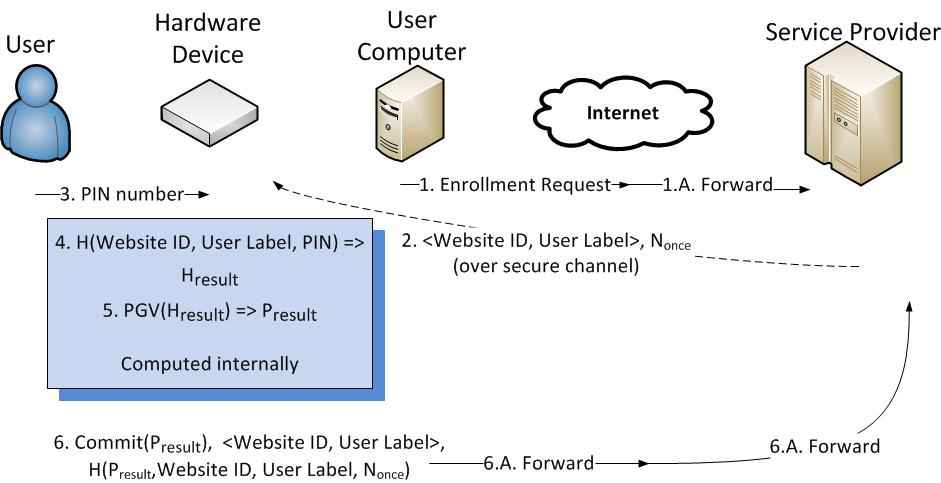
\includegraphics[width=500px]{images/enrollment.jpg}
\label{fig:pearenrollment}
\caption{The enrollment stage of PEAR}
\end{figure}
\FloatBarrier

\begin{figure}[!ht]
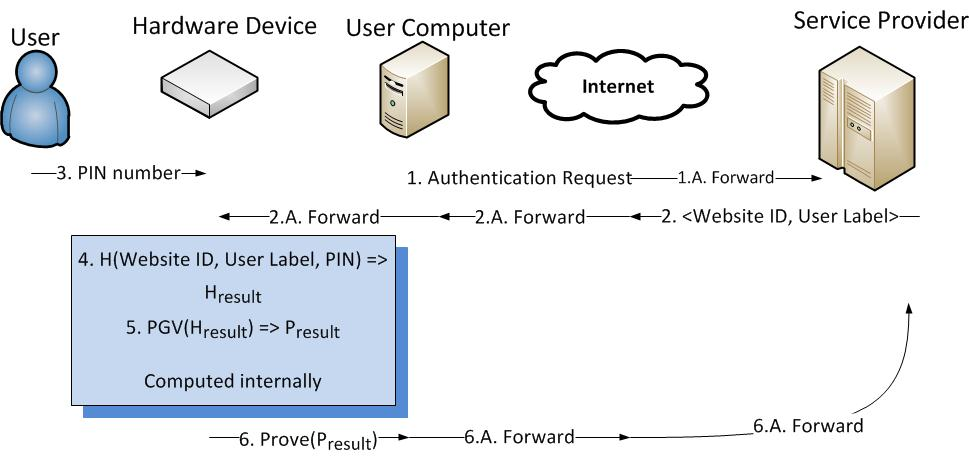
\includegraphics[width=500px]{images/auth.jpg}
\label{fig:pearauthentication}
\caption{The authentication stage of PEAR}
\end{figure}
\FloatBarrier

\begin{table}[!ht]
\label{tab:pearprotocol}
\caption{Formalized version of the PEAR protocols}
\noindent\makebox[\textwidth]{%
\begin{tabular}{|l|}
\hline
{\sf Enroll}($U$) - Device $T$ (using input data from user $U$) computes a commitment and enrolls the results with $S$. \\
\hline
- $C$ requests enrollment from $S$ \\
- $S$ sends the tuple $<$Label, ID$>$ and nonce $N$ to $T$ over a secure channel \\
- $U$ sends PIN to $T$ \\
- $T$ computes {\sf H}(ID, Label, PIN) as $H_{result}$ \\
- $T$ executes {\sf PGV}($H_{result}$) as $P_{result}$ \\
- $T$ sends {\sf Commit}($P_{result}$), $<$Label, ID$>$, {\sf H}({\sf Commit}($P_{result}$),Label,ID,$N$) to $S$, via $C$ \\
\hline
\hline
{\sf Authenticate}($U$) - Device $T$ (using input data from user $U$) authenticates itself as a registered user of $S$. \\
\hline
- $C$ initiates the authentication request from $S$ \\
- $S$ sends the tuple $<$Label, ID$>$ and {\sf Chal}($P_{result}$) to $T$ \\
- $U$ sends PIN to $T$ \\
- $T$ computes {\sf H}(ID, Label, PIN) as $H_{result}$ \\
- $T$ executes {\sf PGV}($H_{result}$) as $P_{result}$ \\
- $T$ responds with {\sf Prove}($P_{result}$), which $C$ forwards to $S$ \\
\hline
\end{tabular}
}
\end{table}
\FloatBarrier

\section{Security Considerations}
Several lemmas are presented below which address various different security aspects of the PEAR system.
Following the lemmas is a discussion of some of the different security issues facing physical systems that
were discussed in Chapter~\ref{chapter:physicalsystems}.

\subsection{Lemmas}


\noindent \textbf{Lemma 1.} \\
\noindent \emph{A man-in-the-middle attacker cannot recover any useful data communicated over the network between the
service provider and the computer.} \\
{\bf Proof:}  The only data that is transmitted between the computer and network is the tuple containing the service
ID and the user's ID initially and then steps of the zero-knowledge proof (see Figures~\ref{fig:enroll} and
\ref{fig:auth}). The tuple will only be sent during authentication, so we can assume that users are already enrolled.
An attacker gains nothing by intercepting the tuple during authentication, since it still requires both the user PIN
number and the device itself to impersonate a user. Intercepting the steps of the zero-knowledge proof also gives him
no information since these zero-knowledge protocols do not reveal any information about the committed value.
%\hfill$\square$ \\

\noindent \textbf{Lemma 2.} \\
\noindent \emph{A man-in-the-middle attacker cannot recover any useful data communicated between the user computer and
the device.} \\
{\bf Proof:}  As shown in Figures~\ref{fig:enroll} and \ref{fig:auth}, the only data that is being transmitted over this channel is
the tuple from the server and the zero-knowledge steps. As shown in Lemma 1, an attacker cannot gain any useful
information from this. 
Also note that the PUF secret is never transferred outside of the device, but rather a commitment or
proof is sent. As such, a MITM attack would not reveal the user's secret, but only the various steps of
the zero-knowledge proofs, which are secure against MITM attacks. In addition, the service provider does not even ever
know the user's PIN.%\hfill$\square$ \\

\noindent \textbf{Lemma 3.} \\
\noindent \emph{An active man-in-the-middle attacker cannot recover any useful information by modifying data between
the device and computer or computer and network during the authentication stage.} \\
{\bf Proof:}  An attacker who modifies the tuple being sent to the device or computer from the network would cause the
device to create an incorrect zero-knowledge proof. This would disrupt the user's ability to authenticate. However,
the attacker would not be able to glean any information from the proof generated from this modified tuple, due to the
use of the zero-knowledge proof.
Note that an attacker would be able to recover useful information if it could modify the tuple during enrollment. It
could substitute a malicious tuple for the valid tuple, which would cause users to be authenticating to the MITM, rather
than the service provider. We avoid this problem by requiring that the tuple be sent securely during enrollment.
%\hfill$\square$ \\

\noindent \textbf{Lemma 4.} \\
\noindent \emph{A PPT adversary can impersonate a legitimate user to the server with only negligible probability.} \\
{\bf Proof:}   As the final authentication step is to complete a zero-knowledge proof, an attacker would have to be able
to defeat a zero-knowledge proof, which happens only with a negligible probability if an attacker does not know the
user's secret.%\hfill$\square$ \\

\noindent \textbf{Lemma 5.} \\
\noindent \emph{Given physical access to the device, an attacker could impersonate the legitimate user with only
negligible probability.} \\
{\bf Proof:}  If an attacker had access to the device, it would not be able to compute the proper hash value unless it
supplied the correct PIN to the device. If the attacker attempted a brute force attack on the user's PIN,
it would be trivial for a server to detect and disable the user's account temporarily. As long as the key space for the
PIN is sufficient, this attack is not realistic.%\hfill$\square$ \\

\noindent \textbf{Lemma 6.} \\
\noindent \emph{A legitimate user can authenticate to a legitimate $S$, except with negligible probability.} \\
{\bf Proof:}  As a legitimate user would have access to the user PIN and a valid tuple from the server, he would be
able to successfully complete the zero-knowledge proof, thus authenticating.%\hfill$\square$ \\

\noindent \textbf{Lemma 7.} \\
\noindent \emph{An attacker cannot enroll using an existing or past user's credentials, except with negligible
probability.} \\
{\bf Proof:} An attacker would be able to capture a user's tuple during authentication. It is plausible that he could
attempt to enroll using this tuple. To prevent this, when the service provider issues the tuple initially, it also
provides a nonce. During the enrollment protocol, the user submits the committed value, the tuple, and a hash of the
tuple, nonce, and committed value. The service provider will verify that this tuple is valid. If the tuple is not
valid or has already been enrolled, the service provider denies the enrollment request.%\hfill$\square$ \\

\subsection{Man in the Middle}

\subsection{Replay Attacks}

\subsection{Impersonation}

\section{Implementation}
From a high level view, Figure~\ref{fig:peararchitecture} describes the architecture of a PEAR enabled device.

\begin{figure}[!ht]
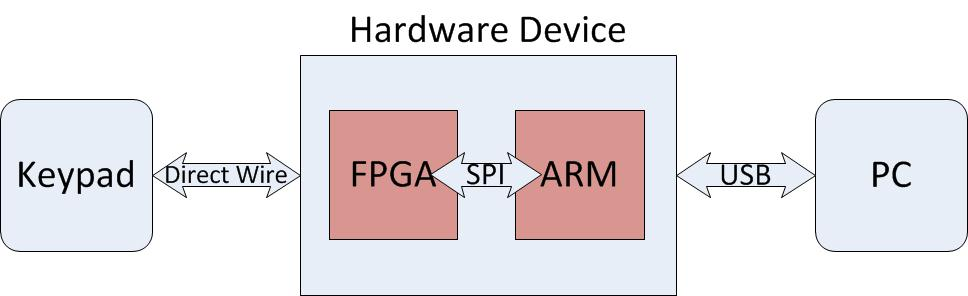
\includegraphics[width=500px]{images/pearimpl.jpg}
\label{fig:peararchitecturet}
\caption{Implementation of a PEAR device}
\end{figure}
\FloatBarrier

\section{Acknowledgement}
This work was partially funded by Sypris Electronics. A paper on PEAR was published in 2010 in the SPRINGL 